\documentclass[10pt, a4paper, oneside, fontset=none]{ctexart}
%调用宏包
\usepackage{amsmath, amsthm, amssymb, graphicx, wrapfig, mathrsfs, upgreek}
\usepackage[bookmarks=true, colorlinks, citecolor=blue, linkcolor=black]{hyperref}
\usepackage{color, framed, geometry, tcolorbox, multirow, booktabs}
\tcbuselibrary{breakable}%box跨页
\tcbuselibrary{skins}%box跨页不留边
%\usepackage{CJKpunct}
\usepackage{marginnote}
\usepackage{makecell, booktabs, longtable}
\usepackage[font=sf, labelfont+=bf]{caption}
\usepackage[font={small, sf}]{subfig}
\usepackage{multicol}
\usepackage{arydshln, nicematrix}%矩阵
\usepackage{extarrows}
\usepackage[american, cuteinductors, ]{circuitikz}
\usepackage{xpatch}
\usepackage{rotating}%旋转
\usepackage{physics}
\usepackage{siunitx}
\usepackage{enumitem}
\usepackage{listings}
\usepackage[text=\includegraphics{C:/Users/16870/.vscode/LaTeX_Application/tex/23Au/图标简稿.png},angle=0]{draftwatermark}%水印
%\usepackage{tikz}
%基本字体设置
\usepackage[math-style=ISO, bold-style=ISO]{unicode-math}
\setmainfont{KpRoman}
%\setmainfont{EB Garamond}
%\setmathfont{Garamond-Math.otf}[StylisticSet={7,9}]
\setmonofont{Iosevka}
\setmathfont{KpMath-Regular.otf}%NewCMMath-Regular
%\setmathfont[range=bb]{TeXGyrePagellaMath-Regular}
%\setmathsfont(Digits,Latin){Garamond MT Pro}
\setCJKmainfont{方正书宋_GBK}[BoldFont={思源宋体 CN Bold}, ItalicFont=方正楷体_GBK, BoldItalicFont={汉仪颜楷W}]
\setCJKsansfont{汉仪文黑-45W ExtraLight}[BoldFont={汉仪文黑-75W Bold}, ItalicFont={方正颜真卿楷书 简繁}]
\setCJKmonofont{LXGWNeoXiHei.ttf}
%附加字体设置
\newCJKfontfamily{\kaico}{可口可乐在乎体 楷体}
\newCJKfontfamily{\kai}{方正楷体_GBK}[BoldFont={汉仪颜楷W}, ItalicFont={方正清刻本悦宋 简繁}, BoldItalicFont={方正颜真卿楷书 简繁}]
\newCJKfontfamily{\yan}{方正清刻本悦宋 简繁}[ItalicFont={方正颜真卿楷书 简繁}]
\newCJKfontfamily{\xiu}{方正宋刻本秀楷_GBK}[ItalicFont={方正宋刻本秀楷_GBK}, BoldFont={方正颜真卿楷书 简繁}]
\newCJKfontfamily{\run}{汉仪润圆-45W}[BoldFont=汉仪润圆-75W, ItalicFont={汉仪润圆-45W}]
\newCJKfontfamily{\wen}{汉仪文黑-45W ExtraLight}[BoldFont={汉仪文黑-75W Bold}, ItalicFont={汉仪文黑-85W Heavy}]
%文档格式
\geometry{left=2.24cm, right=2.24cm, top=3.18cm, bottom=3.18cm}
\linespread{1.4}
\numberwithin{equation}{section}
\setcounter{tocdepth}{3}
\setcounter{secnumdepth}{4}
\renewcommand{\theparagraph}{\hskip2em\Alph{paragraph})}
\newcommand{\Section}[1]{ \refstepcounter{section} \section*{*\thesection\texorpdfstring{\quad}{} #1} \addcontentsline{toc}{section}{\makebox[0pt][r]{*}\thesection\texorpdfstring{\quad}{} #1} }
\newcommand{\Subsection}[1]{ \refstepcounter{subsection} \subsection*{*\thesubsection\texorpdfstring{\quad}{} #1} \addcontentsline{toc}{subsection}{\makebox[0pt][r]{*}\thesubsection\texorpdfstring{\quad}{} #1} }
\newcommand{\Subsubsection}[1]{ \refstepcounter{subsubsection} \subsubsection*{*\thesubsubsection\texorpdfstring{\quad}{} #1} \addcontentsline{toc}{subsubsection}{\makebox[0pt][r]{*}\thesubsubsection\texorpdfstring{\quad}{} #1} }
\setlist[itemize]{leftmargin=3em, labelsep=0.25em, itemindent=0em, itemsep=0pt, parsep=0pt, topsep=3pt, partopsep=0pt}
\setlist[description]{align=left, leftmargin=2em, itemindent=-1em, labelsep=1em, parsep=0pt, topsep=3pt, partopsep=0pt}
\setlength{\marginparwidth}{8em}
\setlength{\lineskip}{5pt}
\setlength{\lineskiplimit}{5pt}

\setlength{\abovecaptionskip}{0.3em}
\setlength{\belowcaptionskip}{0em}
\captionsetup[subfigure]{captionskip=0.5em, nearskip=0em}
\captionsetup[table]{justification=raggedright,singlelinecheck=false}
\renewcommand{\thefigure}{\thesection.\arabic{figure}}
\renewcommand{\thetable}{\thesection.\arabic{table}}

\tikzset{every node/.style={scale=0.8}}
\ctikzset{monopoles/vcc/arrow={Stealth[width=4pt, length=6pt]}}
\ctikzset{monopoles/vee/arrow={Stealth[width=4pt, length=6pt]}}
\ctikzset{bipoles/length=1cm} %电路图大小标的
\ctikzset{resistors/thickness=2.5}
\ctikzset{voltage=raised}
\ctikzset{bipoles/cuteswitch/thickness=0.4}
\tikzset{ %元件着色
    R/.append style={color=balib},
    C/.append style={color=balib},
    L/.append style={color=balib},
    Do/.append style={color=balib},
    zDo/.append style={color=balib},
    leDo/.append style={color=balib},
    pDo/.append style={color=balib},
    battery1/.append style={color=meihong!75!black},
    battery2/.append style={color=meihong!75!black},
    battery/.append style={color=meihong!75!black},
    cI/.append style={color=meihong!75!black},
    I/.append style={color=meihong!75!black},
    cV/.append style={color=meihong!75!black},
    V/.append style={color=meihong!75!black},
}
\tikzset{bcirc/.style={circ, color=black}}
\tikzset{wcirc/.style={ocirc, color=black, fill=white}}
\ctikzset{
	*-*/.style = {bipole nodes={bcirc}{bcirc}},
	-*/.style = {bipole nodes={none}{bcirc}},
	*-/.style = {bipole nodes={bcirc}{none}},
	o-o/.style = {bipole nodes={wcirc}{wcirc}},
	-o/.style = {bipole nodes={none}{wcirc}},
	o-/.style = {bipole nodes={wcirc}{none}},
	o-*/.style = {bipole nodes={wcirc}{bcirc}},
	*-o/.style = {bipole nodes={bcirc}{wcirc}}
}
\newcommand{\bi}[1]{% name
	\node [currarrow, color=black, anchor=center,
	rotate=\ctikzgetdirection{#1-Iarrow}] at (#1-Ipos) {};
}
\newcommand{\bv}[1]{% name
	\draw [color=black] (#1-Vfrom) .. controls (#1-Vcont1)
	and (#1-Vcont2).. (#1-Vto) node [currarrow,
	sloped, anchor=tip, allow upside down,pos=1]{};
}
\renewcommand{\bf}[1]{% name
	\draw [color=black] (#1-Ffrom) -- (#1-Fto) node [currarrow,
	sloped, anchor=tip, allow upside down,pos=1]{};
}
\ctikzset{!vi/.style={no v symbols, no i symbols, no f symbols}}
%\punctstyle{kaiming}
%定理环境
\theoremstyle{plain}
\newtheorem{theorem}{定理}[subsection]
\newtheorem{definition}{定义}[subsection]
\newtheorem{lemma}[theorem]{引理}
\newtheorem{corollary}[theorem]{推论}
\newtheorem{proposition}[theorem]{命题}

\theoremstyle{definition}
\newtheorem{example}[theorem]{例}
\newtheorem{circum}[theorem]{情形}

\newenvironment{proofs}[1][\small\proofname]{\begin{pf}[breakable, enhanced jigsaw]\begin{proof}[#1]\small\kai
	\abovedisplayskip=2pt
	\belowdisplayskip=2pt
}{\end{proof}\end{pf}}
\newenvironment{solution}[1][解]{\begin{proofs}[\small\textit{\yan #1}]\renewcommand{\qedsymbol}{$\circledS$}}{\end{proofs}}
\renewcommand{\proofname}{\yan{证明}}

\renewenvironment{cases}[1][l]{\left\{\,\begin{NiceArray}{#1}}{\end{NiceArray}\right.}
%颜色命名
\definecolor{meihong}{rgb}{0.85,0.2,0.47}
\definecolor{bali}{rgb}{0.2,0.6,0.78}
\definecolor{qinglv}{rgb}{0,0.35,0.32}
\definecolor{meihongb}{rgb}{0.85,0.2,0.47}
\definecolor{balib}{rgb}{0.15,0.45,0.58}
\definecolor{qinglvb}{rgb}{0,0.35,0.32}
%box环境
\newtcolorbox{pr}[2][]
{colback=black!5!white,colframe=white!75!black,fonttitle=\sffamily\wen\bfseries,title=#2,#1}
\newtcolorbox[use counter=definition,number within=subsection]{defi}[2][]
{colback=bali!5!white,colframe=bali!75!black,fonttitle=\sffamily\wen\bfseries,title=定义~\thetcbcounter. #2,#1}
\newtcolorbox[auto counter,number within=section]{compl}[2][]
{colback=bali!5!white,colframe=bali!65!black,fonttitle=\sffamily\wen\bfseries,label=#2,title=元件~\thetcbcounter. #2,#1, fontupper=\kai, fontlower=\kai}
\newtcolorbox[use counter=theorem,number within=subsection]{theo}[2][]
{%grow to right by=3.2cm,
colback=meihong!5!white,colframe=meihong!75!black,fonttitle=\sffamily\wen\bfseries,fontupper=\run,title=结论~\thetcbcounter. #2,#1}
\newtcolorbox[use counter=definition,number within=subsection]{defil}[2][]
{colback=bali!5!white,colframe=bali!75!black,fonttitle=\sffamily\wen\bfseries,label=#2,title=定义~\thetcbcounter. #2,#1}
\newtcolorbox[use counter=theorem,number within=subsection]{theol}[2][]
{%grow to right by=3.2cm,
colback=meihong!5!white,colframe=meihong!75!black,fonttitle=\sffamily\wen\bfseries,fontupper=\run,label=#2,title=结论~\thetcbcounter. #2,#1}
\newtcolorbox[auto counter,number within=section]{note}[2][]
{colback=qinglv!5!white,colframe=qinglv!75!black,fonttitle=\sffamily\wen\bfseries,title=注~\thetcbcounter. #2,#1}
\newtcbox{\prenote}[1][]
{left=0.25em,right=0.25em,top=0.25em,bottom=0.25em,width=8.5em,toptitle=0.1em,before skip=0pt,after skip=3pt,colback=gray!5!white,colframe=gray!50!black,fonttitle=\linespread{1}\raggedright\small\sf\bfseries,fontupper=\linespread{1}\small\sf,title=#1}
\newtcolorbox{pf}[1][]
{colback=black!5!white,colframe=white!75!black,#1}
\newtcolorbox{eq}[1][]
{standard jigsaw, colback=meihong!5!white, opacityback=0.7, %grow to right by=3.2cm, 
colframe=meihong!85!black,#1, boxrule=0.4pt, leftrule=10pt, arc=0pt, before skip=7pt, after skip=7pt}
%\newcommand{\mybox}[1]{\tikz[baseline=(MeNode.base)]{\node[rounded corners, fill=gray!20](MeNode){#1};}}

\lstset{
	xleftmargin=3em, xrightmargin=1em, 
	breaklines,                                 % 自动将长的代码行换行排版
	extendedchars=false,                        % 解决代码跨页时,章节标题,页眉等汉字不显示的问题
	rulecolor=\color[rgb]{0.8,0.8,0.8},         % 设置代码框颜色
	backgroundcolor=\color[rgb]{0.96,0.96,0.96},% 背景颜色
	keywordstyle=\colors{bali}\bfseries,        % 关键字颜色
	identifierstyle=\color{black},              % 普通标识符颜色
	commentstyle=\rm\kai\color{gray},          	% 注释颜色
	stringstyle=\colors{meihong},      			% 字符串颜色
	showstringspaces=false,                     % 不显示字符串内的空格
	numbers=left,                               % 显示行号
	numberstyle=\tiny,              			% 设置数字字体
	basicstyle=\linespread{1}\tt,               % 设置基本字体
	captionpos=t,                               % title在上方(在bottom即为b)
	frame=single,                               % 设置代码框形式
	showtabs=false, 
	numbersep=15pt, 
	framesep=1em, 
	language=C++, 
	columns=flexible, 
	tabsize=4, 
}

\catcode`\,=\active
\def ,{\textup{,}\hskip0.5em }
\newcommand{\hang}[1][1]{\hangafter 1 \hangindent #1em \noindent}
\newcommand{\page}[1]{\hfill P$_\text{#1}$}
\newcommand{\colors}[1]{\color{#1!75!black}}
\newcommand{\paratitle}[1]{\hang \textbf{\wen #1}\hskip1em}
\newcommand{\tboqi}[1]{\textbf{\xiu\color{qinglv!75!black}#1}}
\newcommand{\mboqi}[1]{\symbf{\xiu\color{qinglv!75!black}#1}}
\newcommand{\tboba}[1]{\textbf{\kai\color{bali!75!black}#1}}
\newcommand{\mboba}[1]{\symbf{\kai\color{bali!75!black}#1}}
\newcommand{\tbome}[1]{\textbf{\run\run\color{meihong!75!black}#1}}
\newcommand{\mbome}[1]{\run\symbf{\run\color{meihong!75!black}#1}}
\newcommand{\adjline}{	\lineskiplimit=3pt
	\lineskip=3pt
	\abovedisplayskip=6pt
	\belowdisplayskip=6pt 
	}
\newcommand{\den}[2][]{\begin{defi}{#1}\adjline
	\kai #2\end{defi}}
\newcommand{\din}[2][]{\begin{theo}{#1}\adjline
	\run #2\end{theo}}
\newcommand{\de}[2][]{\begin{defil}{#1}\adjline
	\kai #2\end{defil}}
\newcommand{\di}[2][]{\begin{theol}{#1}\adjline
	\run #2\end{theol}}
\newcommand{\dep}[3][]{\begin{defi}{#1\page{#2}}\adjline
	\kai #3\end{defi}}
\newcommand{\dip}[3][]{\begin{theo}{#1\page{#2}}\adjline
	\run #3\end{theo}}
\newcommand{\zhu}[2][]{\begin{note}{#1}\adjline
	\xiu #2\end{note}}
\newcommand{\bu}[3][]{\begin{compl}{#1}	\paratitle{记号}#2 \tcblower\paratitle{特性}#3\end{compl}}
\newcommand{\trans}[2][注]{\begin{wrapfigure}{r}{8.7em}
		\vspace{-1.5em}
		\prenote[#1]{\makebox[8em][l]{#2}}
	\end{wrapfigure}}
% \newcommand{\tranS}[3][-1]{\marginnote{
% 		\begin{prenote}{#2}
% 			\raggedright
% 			#3
% 		\end{prenote}
% 	}[#1\baselineskip]}
\newcommand{\cbox}[2][]{
	$\vcenter{\hbox{\begin{circuitikz}[#1]
		#2
	\end{circuitikz}}}$
	}
\newcommand{\shbox}[1]{\cbox{\draw (0,0) to[#1] (1.5,0);}(\texttt{#1})}
%定义算符
\newcommand{\rref}{\symup{rref}}
\newcommand{\C}{\mathbb{C}}
\renewcommand{\i}{\symsf{j}}
\newcommand{\neiji}[4]{\symbf{#1}_{#3}^\symup{T}\symbf{#2}_{#4}}
\def\upint{\mathchoice%
	{\mkern13mu\overline{\vphantom{\intop}\mkern7mu}\mkern-20mu}%
	{\mkern7mu\overline{\vphantom{\intop}\mkern7mu}\mkern-14mu}%
	{\mkern7mu\overline{\vphantom{\intop}\mkern7mu}\mkern-14mu}%
	{\mkern7mu\overline{\vphantom{\intop}\mkern7mu}\mkern-14mu}%
	\int}
\def\lowint{\mkern3mu\underline{\vphantom{\intop}\mkern7mu}\mkern-10mu\int}
\renewcommand{\a}[1]{\left\langle #1 \right\rangle}
\renewcommand{\v}{\vee}
\newcommand{\A}{\wedge}
\renewcommand{\c}[1]{\symbfsfit{#1}}
\newcommand{\V}{\c{V}}
\newcommand{\I}{\c{I}}
\newcommand{\G}{\c{G}}
\newcommand{\Lr}{\Leftrightarrow}
\newcommand{\LLr}[2][]{\xLongleftrightarrow[#1]{#2}}
\newcommand{\rl}{\rightleftarrows}
\newcommand{\dif}{\mathop{}\!\symup{d}}
\newcommand{\Dif}{\mathop{}\!\symup{\Delta}}
\newcommand{\e}{\symup{e}}
\newcommand{\R}{\mathbb{R}}
\newcommand{\bF}{\mathbb{F}}
\newcommand{\dint}{\displaystyle\int}
\newcommand{\dt}[1][]{\dfrac{\dif #1}{\dif t}}
\renewcommand{\ang}[1]{\vcenter{\hbox{\begin{tikzpicture}
	\node (box) at (0,0) {$#1$};
	\draw (box.south west) ++ (-0.05,0.08) coordinate(left)
	(box.south east) ++ (-0.1,0.08) -- (left) -- ++ (0.17,0.45);
\end{tikzpicture}}}\!\!}
\newcommand{\meshcurrent}[2]{\draw[latex-] #1 node{#2} +(0.43,0.25) arc(30:330:0.5);
}
\newcommand{\equ}[1]{\begin{eq}
%	\setmathfont{GFSNeohellenicMath.otf}
	\setmathfont{FiraMath-Regular.otf}\sffamily
	\begin{equation}
		{\color{meihong!85!black} #1}
	\end{equation}\end{eq}
\setmathfont{KpMath-Regular.otf}
}
\newcommand{\mrm}[1]{{\symup{#1}}}
\newcommand{\uni}[1]{{\symup{\,#1}}}
%\setmathfont{Garamond-Math.otf}[StylisticSet={7,9}]}
%标题、作者、日期
\title
{
	\textbf{Basic Engineering Circuit Analysis\\电子电路启蒙教程}
}
\author{\zihao{5} T$^\text{T}$T}
\date{\zihao{5} \kai \today}
%----------------------------------------------------------
\begin{document}

\adjline

\maketitle
\begin{multicols}{2}
	\begin{flushleft}
		\tableofcontents
	\end{flushleft}
\end{multicols}

%\newgeometry{left=2.24cm, right=5.14cm, top=3.18cm, bottom=3.18cm}
\newpage
\setcounter{section}{3}
%----------------------------------------------------------
\section{非线性器件}

\subsection{\textsl{pn}结与二极管}

\subsubsection{\textsl{p}型半导体与\textsl{n}型半导体}

硅晶体中,在0 K下每个硅原子周边成4根共价键,价电子全部约束在共价键内,称为\textbf{本征硅};温度升高,电子逃逸成为\textbf{自由电子}(\textsl{n}),在其母原子周围留下\textbf{空穴}(\textsl{p})。当加上电场时,自由电子将定向移动,空穴临近位置的约束电子也可能填补空穴,在其原位置产生新的空穴,形成空穴的「移动」。因此,在半导体中有两种\tboba{载流子}:带一个单位负电荷的自由电子,和带一个单位正电荷的空穴。其中含量多的称为\tboba{多数载流子},简称\tboba{多子};含量少的称为\tboba{少数载流子},简称\tboba{少子}。
\begin{figure}[ht!]
	\begin{center}
	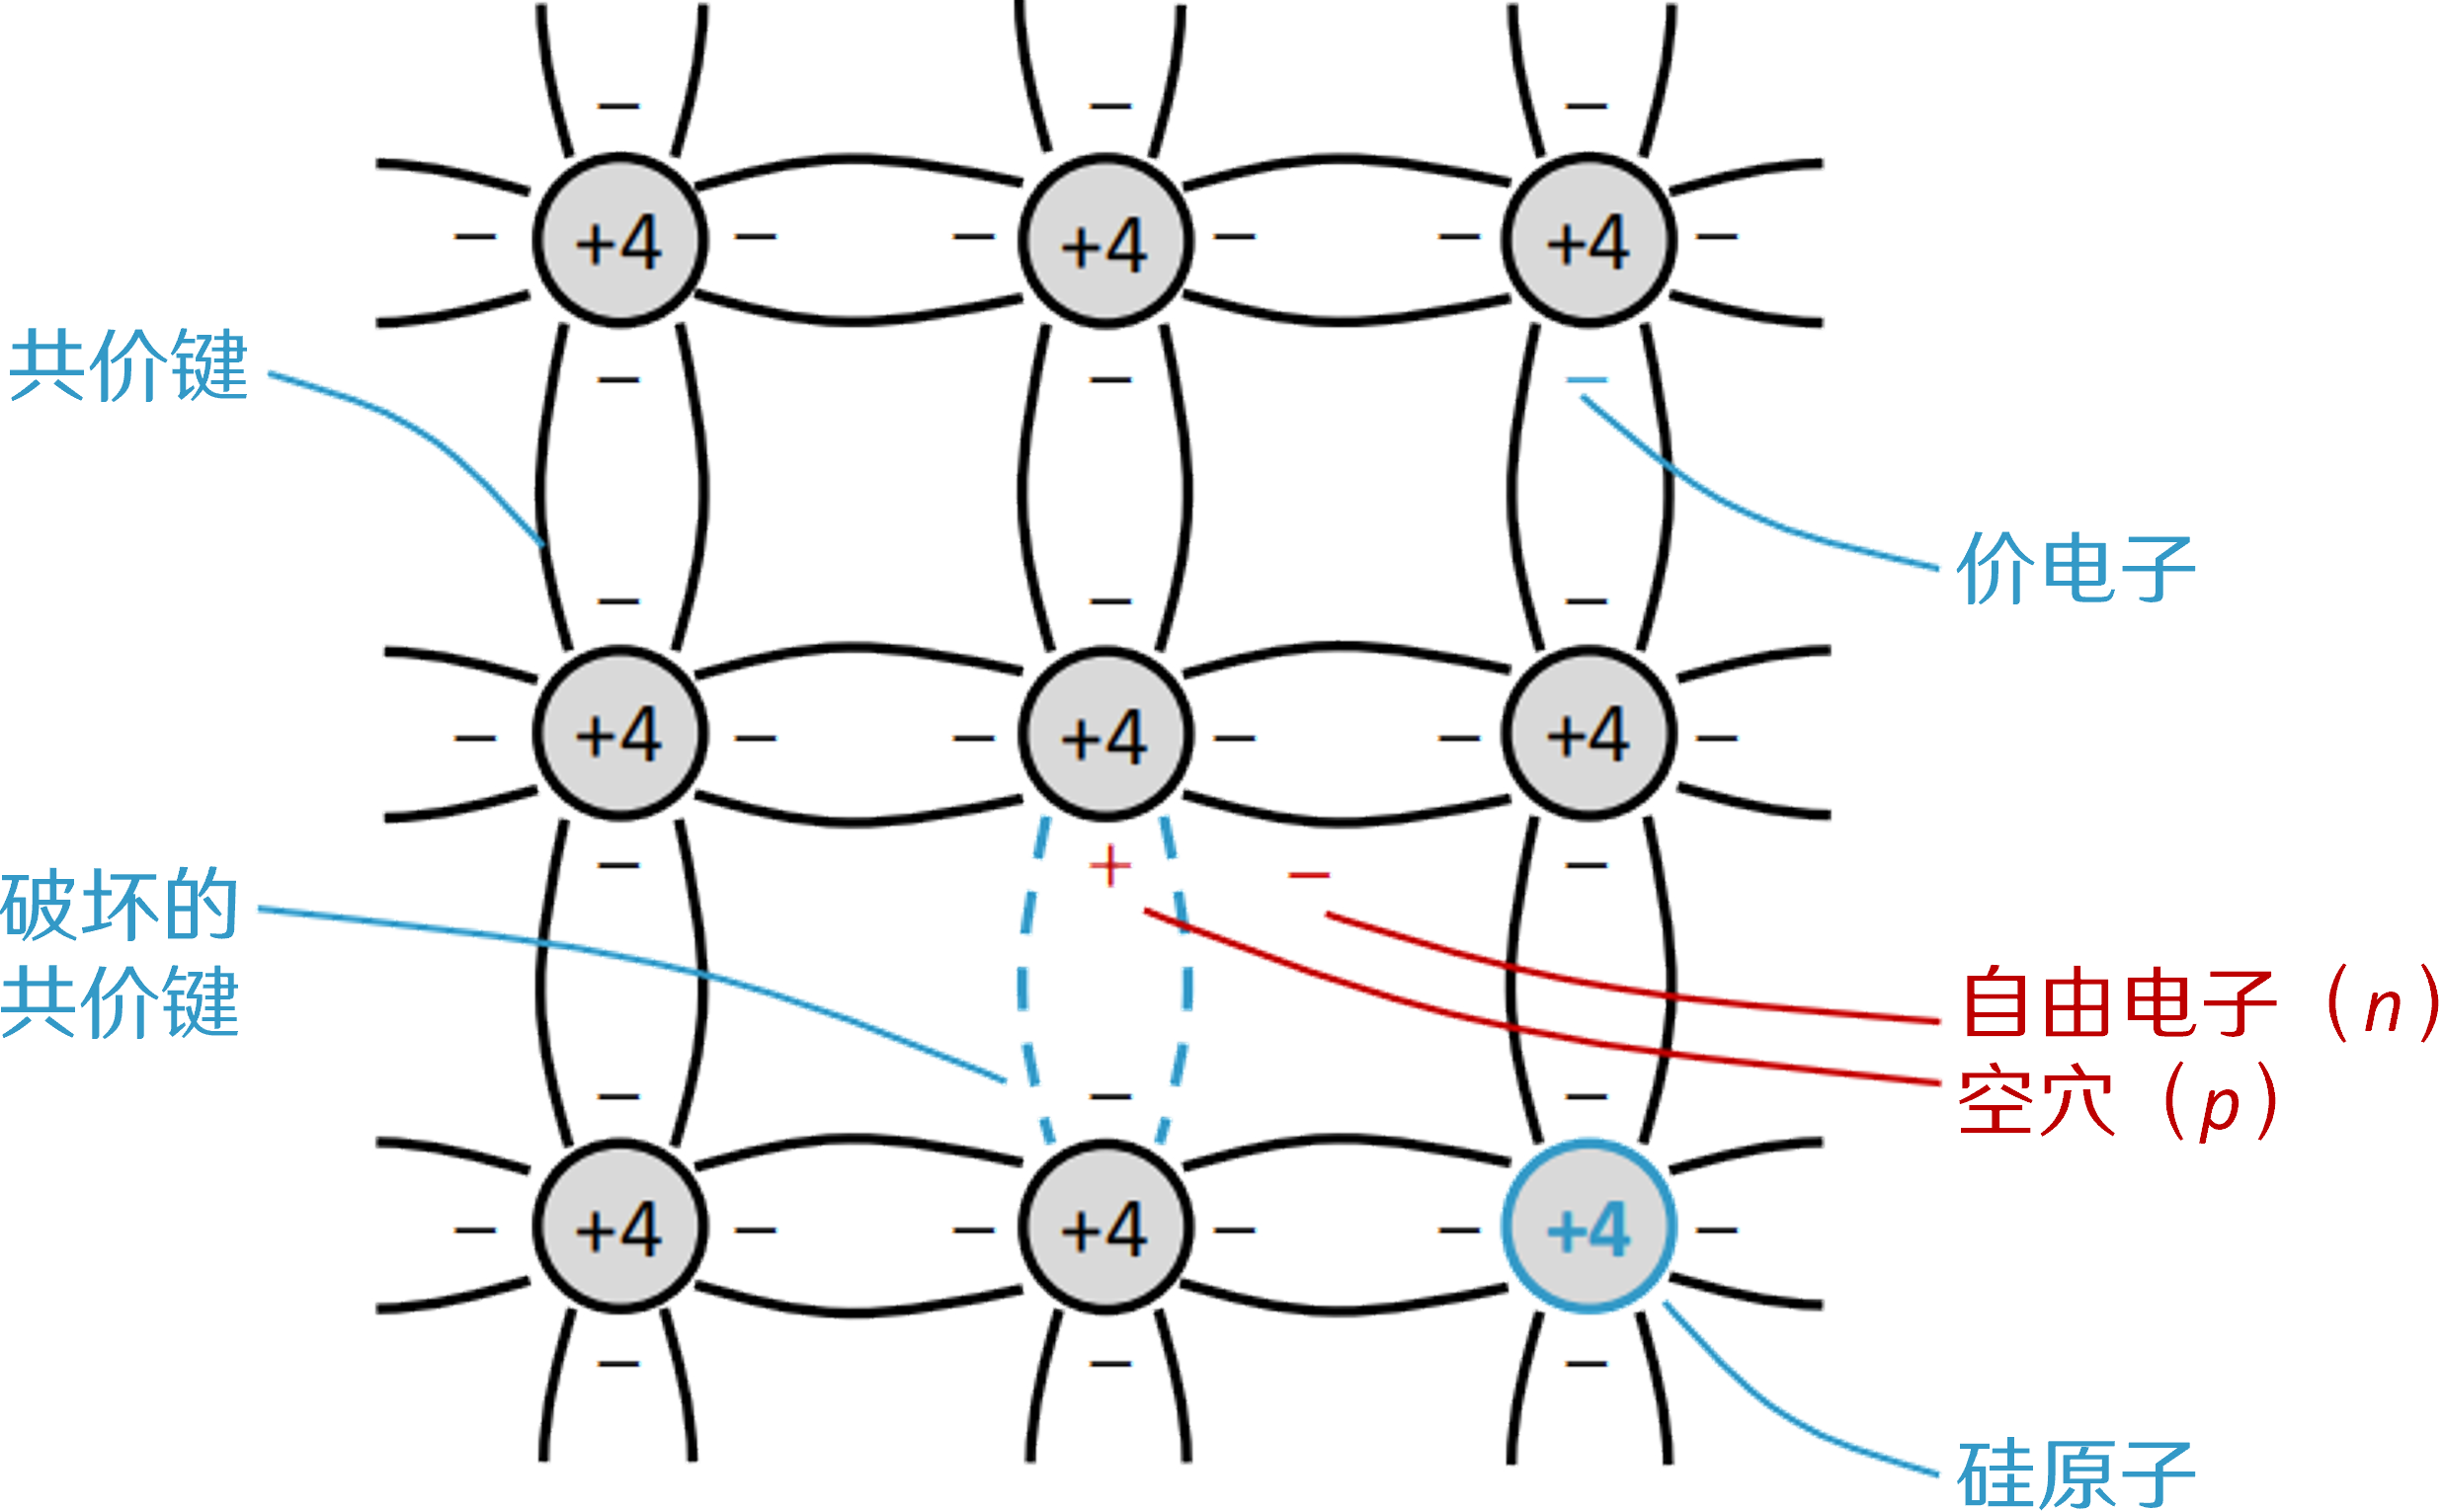
\includegraphics[width=10cm]{半导体载流子.png}
	\caption{半导体中的载流子}\label{Pic: Semiconductor carriers}
	\vspace{-1.5em}
	\end{center}
\end{figure}

但纯硅晶体中载流子的浓度太低,无法传导明显的电流。为提高载流子的浓度,往往对硅晶体\textbf{掺杂},即引入价电子数不同的杂质原子。
\begin{itemize}
	\item 引入5价原子(如P),每个杂质原子可额外贡献一个自由电子,会使自由电子浓度增大,形成~\tboba{\textsl{n}型半导体}。\textsl{n}型半导体中,多子为自由电子,少子为空穴。
	\item 引入3价原子(如B),每个杂质原子可从临近原子接受一个电子,从而额外产生一个空穴,形成~\tboba{\textsl{p}型半导体}。\textsl{p}型半导体中,多子为空穴,少子为自由电子。
\end{itemize}

\trans[漂移电流]{drift current}
半导体中载流子(自由电子和空穴)的运动产生电流。由电场作用产生的电流称为\tboba{漂移电流},其电流密度与载流子的电荷量、浓度、迁移率成正比,即有 
$$J_\textsl{p}=q_ep\mu_\textsl{p}E,\qquad J_\textsl{n}=q_en\mu_\textsl{n}E$$
其中$p$和$n$就分别是空穴和自由电子的浓度,$\mu_\textsl{p}$和$\mu_\textsl{n}$分别是空穴和自由电子的迁移率,而总电流密度就是
$$J=J_\textsl{p}+J_\textsl{n}=q_e(p\mu_\textsl{p}+n\mu_\textsl{n})E$$
即电导率为$\sigma=\dfrac{J}{E}=q_e(p\mu_\textsl{p}+n\mu_\textsl{n})$。

由载流子顺浓度梯度的扩散产生的电流称为\tboba{扩散电流},其电流密度与载流子的电荷量、扩散常数和浓度梯度成正比,即有
$$J_\textsl{p}=-q_e D_\textsl{p} \nabla p,\qquad J_\textsl{n}=-q_e D_\textsl{n} \nabla n$$
其中$D_\textsl{p}$和$D_\textsl{n}$分别是空穴和自由电子的扩散常数,满足
$\dfrac{D_\textsl{n }}{\mu_\textsl{n }}=\dfrac{D_\textsl{p }}{\mu_\textsl{p }}=V_T$,这个比值称为\tboba{热电压},其值为$V_T = \dfrac{kT }{q_e}$,其中$k \approx 1.3806488 \times 10^{-23} \,\symup{J/K}$为Boltzmann常数。温度取$300 \,\symup{K}$时,热电压的值为$2.585 \cp 10^{-2} \,\symup{V}$。

\subsubsection{\textsl{pn}结}

将\textsl{p}型半导体与\textsl{n}型半导体靠在一起,接触位置会发生两种载流子的扩散:空穴向\textsl{n}型半导体扩散,自由电子向\textsl{p}型半导体扩散,使得\textsl{n}型半导体一侧电势稍高于\textsl{p}型半导体一侧,形成\tboba{耗尽层}并建立起电场。该电场会在耗尽层产生\tboba{势垒电压},其值为
$$V_0 =V_T\ln\dfrac{N_AN_D}{n_i^2}$$
其中$N_A$和$N_D$分别是\textsl{p}型半导体与\textsl{n}型半导体中的掺杂浓度。该电压会阻碍空穴和自由电子的扩散,因此需要加上直流偏压。

\paragraph{正向偏置电压} 外加电场的方向与内建电场的方向相反。此时,外加电压将使得耗尽层\textsl{n}侧正电荷减少,\textsl{p}侧负电荷减少,耗尽层变薄。同时,\textsl{p}型半导体中空穴增多,\textsl{n}型半导体中自由电子增多,因而顺外加电压方向可以产生较大的扩散电流。

\paragraph{反向偏置电压} 外加电场的方向与内建电场的方向相同。

\subsubsection{\textsl{pn}结二极管}

\bu[二极管(diode)]{
	\shbox{Do}
}{
	具有单向导通性,伏安特性为$i=I_S\left(\e^\frac{v}{V_T}-1\right)$($v \ge 0$)。
}
这个伏安特性近似也可以写成$v \approx V_T\ln \dfrac{i }{I_S}$($i \ge 0$)。在基尔霍夫定律方程中出现这样的项,往往会将线性方程变为没有解析解的超越方程。因而,需要对二极管进行线性建模。

\paragraph{恒压降模型}

认为导通后电流随电压变化极快,各电流对应电压视作常量$v_D$。则导通后,二极管可视为一个顺导通方向恒有$v_D$压降的直流恒压源。

\paragraph{小信号模型}

1

\bu[齐纳二极管]{
	\shbox{zDo}
}{
	在反向「breakdown」区工作。
}

\subsubsection{特殊的二极管}

\bu[发光二极管(LED)]{
	\shbox{leDo}
}{
	具有二极管的一般特性,同时导通时将电信号转化为光信号。
}
\bu[光电二极管(photodiode)]{
	\shbox{pDo}
}{
	
}


\subsection{双极结式晶体管(BJT)}

\ctikzset{transistors/scale=1.3, color=balib}

\bu[BJT]{
	\textsl{npn}型BJT记为$\vcenter{\hbox{\begin{circuitikz}
		\draw (0,0) -- (0.3,0) node[npn,anchor=B](NPN){} (NPN.C) -- ++(0.3,0) (NPN.E) -- ++(0.3,0);
	\end{circuitikz}}}$(\texttt{npn}),\textsl{pnp}型BJT记为$\vcenter{\hbox{\begin{circuitikz}
		\draw (0,0) -- (0.3,0) node[pnp,anchor=B](NPN){} (NPN.C) -- ++(0.3,0) (NPN.E) -- ++(0.3,0);
	\end{circuitikz}}}$(\texttt{pnp})。
}{
	见~\ref{BJT的端口特性}~节。
}

\subsubsection{BJT的结构与原理}

如图~\ref{Pic: npn型BJT的横截面},\textsl{npn}型BJT由三个半导体区域组成:\tboba{发射极}区(E,\textsl{n}型)、\tboba{基极}区(B,\textsl{p}型)和\tboba{集电极}区(C,\textsl{n}型)。\textsl{pnp}型BJT各区域的半导体材料相反。相邻两个区域相接构成\textsl{pn}结,即形成\tboba{发射结}(EBJ)和\tboba{集电结}(CBJ)。

\begin{figure}[ht!]
	\vspace{-1em}
	\centering
	\subfloat[]{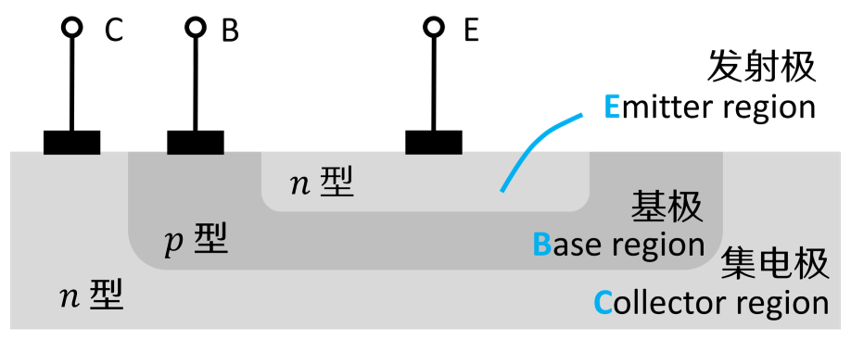
\includegraphics[width=7.51cm]{npn结构.png}}
	\qquad
	\subfloat[]{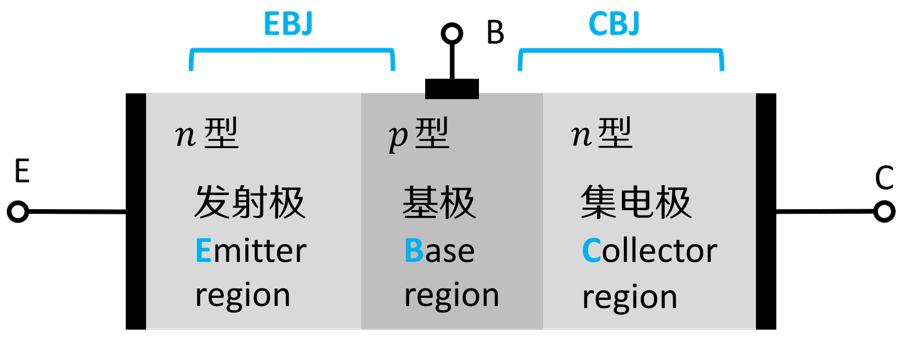
\includegraphics[width=7.95cm]{npn简化结构.png}}
	\caption{\textsl{npn}型BJT的横截面结构示意图}\label{Pic: npn型BJT的横截面}
	\vspace{-1em}
\end{figure}

按照两个\textsl{pn}结的通断特性,BJT有如表~\ref{Tab: BJT的工作模式}~所示的四种工作模式。下面以\textsl{npn}型BJT为例,对它的各模式电路进行分析。

\begin{table}[ht!]
	\caption{BJT的工作模式}\label{Tab: BJT的工作模式}
	\begin{tabular}{p{110pt}<{\centering}p{60pt}<{\centering}p{60pt}<{\centering}}
		\toprule
		\textbf{模式} & \textbf{EBJ} & \textbf{CBJ} \\
		\midrule
		截止Cutoff & 反偏电压 & 反偏电压 \\
		饱和Saturation & 正偏电压 & 正偏电压 \\
		正激活Active & 正偏电压 & 反偏电压 \\
		反激活Reverse active & 反偏电压 & 正偏电压 \\
		\bottomrule
	\end{tabular}
	\vspace{-1em}
\end{table}

\paragraph{正激活Active模式}EBJ上有正向偏压,CBJ上有反向偏压,即$v_{BE}>0,v_{BC}<0$。其集电极电流$i_C$、基极电流$i_B$、发射极电流$i_E$分别为
\equ{
	\begin{aligned}
	&i_C=I_S \e^\frac{v_{BE}}{V_T},&&\qquad \text{其中}\, I_S=\dfrac{A_EqD_nn_i^2}{N_AW}\\[-7pt]
	&i_B=\dfrac{i_C }{\beta_F}=\dfrac{I_S}{\beta_F} \e^\frac{v_{BE}}{V_T}\\
	&i_E=\dfrac{i_C }{\alpha_F}=\dfrac{I_S}{\alpha_F} \e^\frac{v_{BE}}{V_T} ,&&\qquad \text{其中}\, \alpha_F=\dfrac{\beta_F}{\beta_F+1}	
	\end{aligned}
}
\noindent 其电路可有等效替代如下:
\begin{center}
	\cbox{
		\draw (0,0) coordinate(C) to[battery, v_=$v_{CB}$, -*] ++(0,-1.5) coordinate(B) to[battery1, v_=$v_{BE}$] ++(0,-1.5) coordinate(E)
		(B) to[short, -o] ++(1,0) node[below]{B} to[short, o-] ++(0.5,0) node[npn, anchor=B](BJT){}
		(C) -- (C -| BJT.C) to[short, -o] ++(0,-0.5) node[right]{C} to[short, o-] (BJT.C)
		(E) -- (E -| BJT.E) to[short, -o] ++(0,0.5) node[right]{E} to[short, o-] (BJT.E);
	}
	$\Longleftrightarrow$
	\cbox{
		\draw (0,0) coordinate(C) 
		to[battery, v_=$v_{CB}$, -*] ++(0,-1.5) coordinate(B) 
		to[battery1, v_=$v_{BE}$] ++(0,-1.5) coordinate(E)
		(B) 
		to[short, -o] ++(1,0) node[below]{B} 
		to[short, o-, f=$i_B$] ++(0.5,0) 
		to[short, -*] ++(0.4,0) coordinate(BJT)
		(C) 
		-- (C -| BJT) 
		to[short, -o] ++(0,-0.3) node[left]{C} 
		to[cI, o-, l=$\alpha_F i_E$, f>^=$i_C$, !vi, name=iC] (BJT)
		(BJT) 
		to[Do, -o, l=$D_E$, f^>=$i_E$, !vi, name=iE] ++(0,-1.2) node[left]{E} 
		to[short, o-] (E -| BJT) -- (E);
		\bf{iC}\bf{iE}
	}
\end{center}
公式中,$\beta_F$的典型值在50~200之间,则$\alpha_F \approx 1$。

\paragraph{反激活Reverse active模式}EBJ上有反向偏压,CBJ上有正向偏压,即$v_{BE}<0,v_{BC}>0$。其集电极电流$i_C$、基极电流$i_B$、发射极电流$i_E$的关系与上面类似,即
\equ{
	\begin{aligned}
	&i_E=I_S \e^\frac{v_{BC}}{V_T},&&\qquad \text{其中}\, I_S=\dfrac{A_EqD_nn_i^2}{N_AW}\\[-7pt]
	&i_B=\dfrac{i_E }{\beta_R}=\dfrac{I_S}{\beta_R} \e^\frac{v_{BC}}{V_T}\\
	&i_C=\dfrac{i_E }{\alpha_R}=\dfrac{I_S}{\alpha_R} \e^\frac{v_{BC}}{V_T} ,&&\qquad \text{其中}\, \alpha_R=\dfrac{\beta_R}{\beta_R+1}	
	\end{aligned}
}
\noindent 不同的是,$\alpha_R$约为0.01~0.05。

\paragraph{饱和Saturation模式}EBJ、CBJ上均是正向偏压,即$v_{BE}>0,v_{BC}>0$。此时有
\equ{
	i_C=\left(\alpha_F-\dfrac{1}{\alpha_R}\right)I_S \left(\e^\frac{v_{BC}}{V_T}-1\right)+\alpha_Fi_E
}
\noindent 可见当$v_{BC}$增大时,由$\alpha_F-\dfrac{1}{\alpha_R}<0$,知$i_C$减小。

\subsubsection{BJT的端口特性}\label{BJT的端口特性}

\paragraph{BJT的伏安特性}

显见其服从基尔霍夫定律。此外,由上面分析可知三个端口电流的关系,以下即仅分析$i_C$。

\begin{description}
	\item[$\symbf{i_C-v_{BE}}$特性] 
	由$i_C=I_S\e^{v_{BE}/V_T}$可直接得出。

	\item[$\symbf{i_C-v_{CB}}$特性]
	固定$i_E$,Active模式下,$i_C=I_S\e^{v_{BE}/V_T}$与$v_{CB}$无直接关系,$i_C-v_{CB}$曲线是一条与$i_C$轴交于$\alpha_Fi_E$处的水平线;反号后$v_{BC}$继续增大进入Saturation模式,当$v_{BC}$增大时,由$\alpha_F-\dfrac{1}{\alpha_R}<0$,知$i_C=\left(\alpha_F-\dfrac{1}{\alpha_R}\right)I_S \left(\e^{v_{BC}/V_T}-1\right)+\alpha_Fi_E$减小。此外,当$v_{CB}$过大致使反偏\textsl{pn}结击穿时,$i_C$即随$v_{CB}$增大。

	\item[$\symbf{i_C-v_{CE}}$特性]
	固定$i_E$(也即固定$v_{BE}$),由$v_{CE}=v_{BE}+v_{CE}$,容易得到$i_C-v_{CE}$特性曲线与$i_C-v_{CB}$曲线的关系。
\end{description}

\begin{figure}[ht!]
	\vspace{-1em}
	\centering
	\subfloat[$i_C-v_{BE}$]{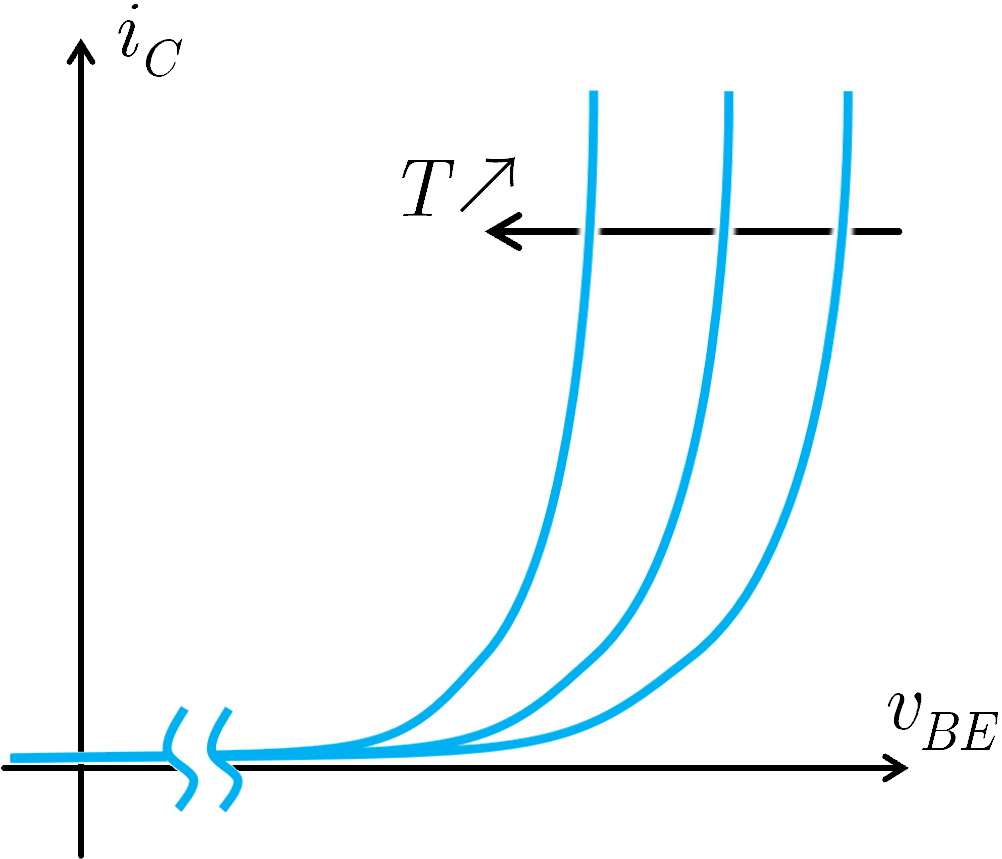
\includegraphics[width=3.87cm]{BJT_iC-vBE.png}}
	\subfloat[$i_C-v_{CB}$]{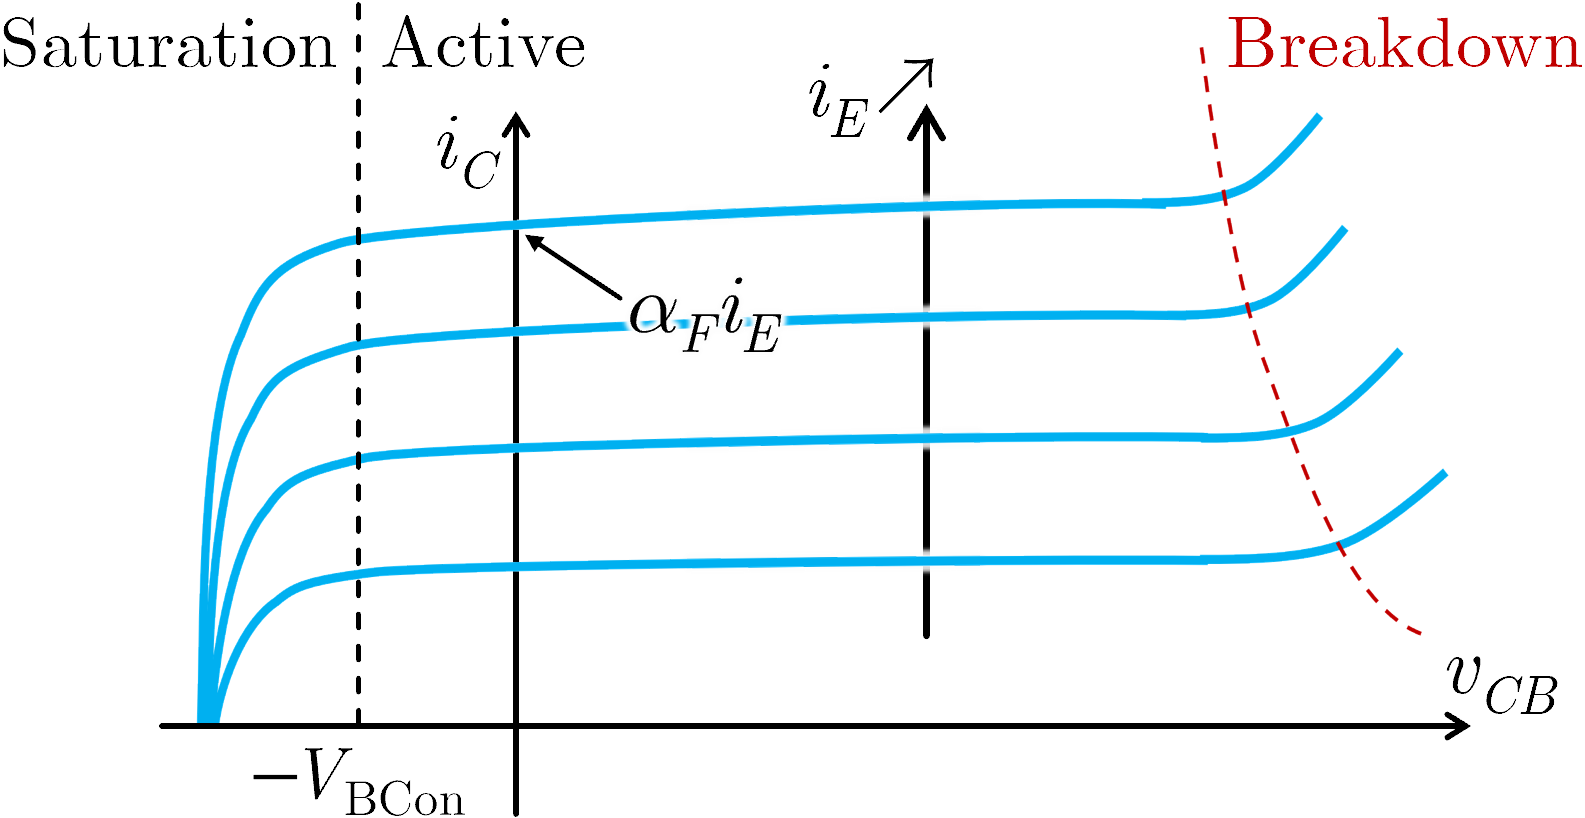
\includegraphics[width=6.14cm]{BJT_iC-vCB.png}}
	\subfloat[$i_C-v_{CE}$]{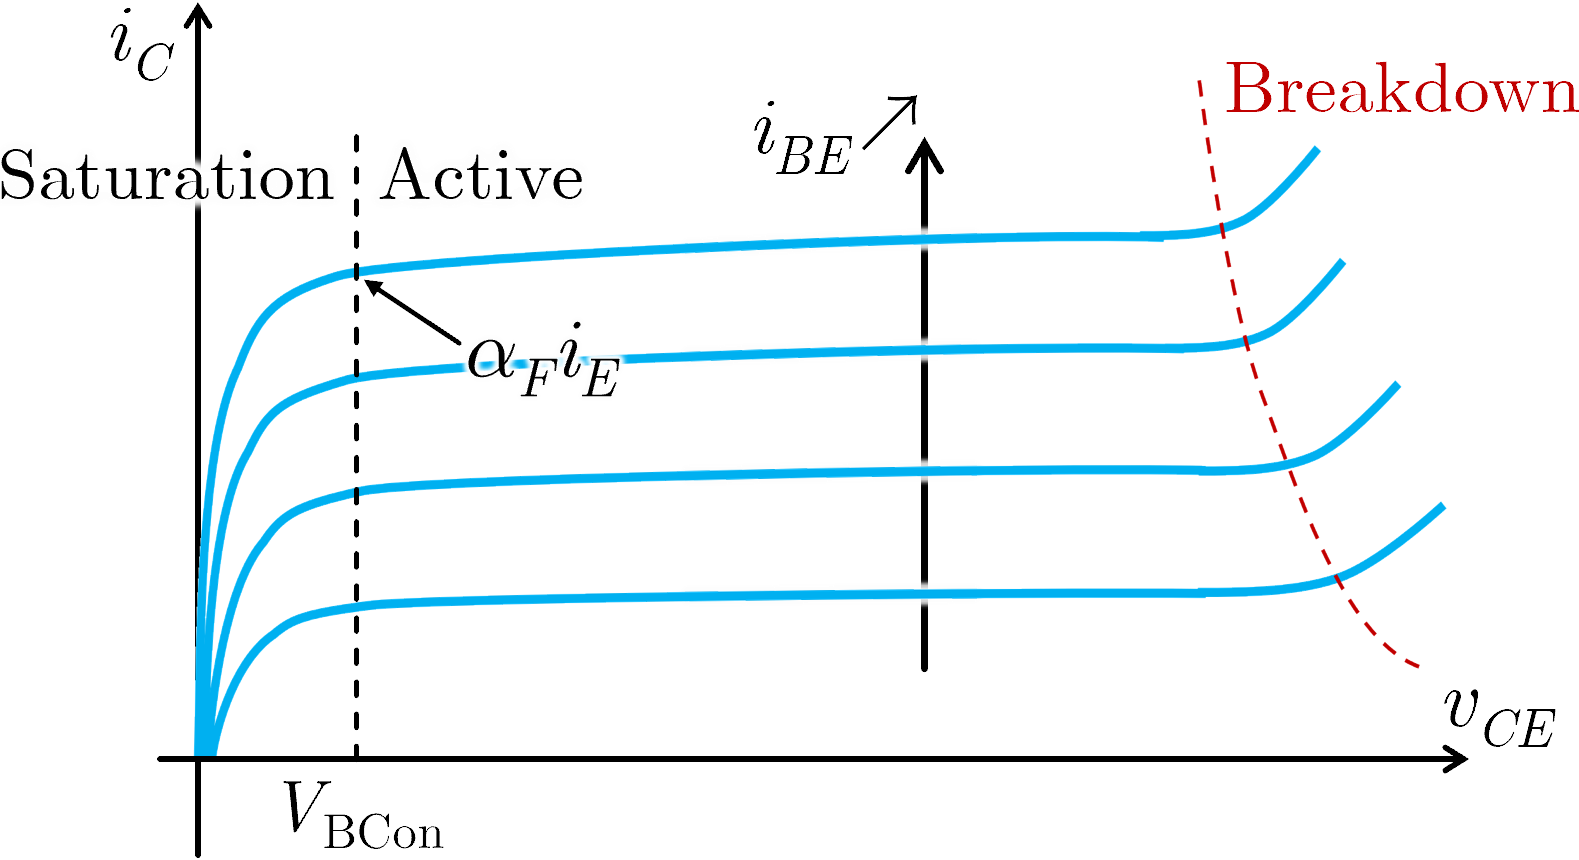
\includegraphics[width=6.14cm]{BJT_iC-vCE.png}}
	\caption{\textsl{npn}型BJT的伏安特性曲线}
	\vspace{-1em}
\end{figure}

实际上,\textsl{npn}型BJT的$i_C-v_{CE}$特性曲线没有上面那么完美,在Active模式区域其并不水平,而是有轻微的上翘,即Active模式下$i_C$仍是与$v_{CE}$有关的:
\equ{
	i_C=I_S\e^\frac{v_{BE}}{V_T}\left(1+\dfrac{v_{CE}}{V_A}\right)
}
\noindent 式中$V_A$称为\textbf{Early电压},这个现象称为~\tbome{Early效应}。

\begin{figure}[ht!]
	\centering
	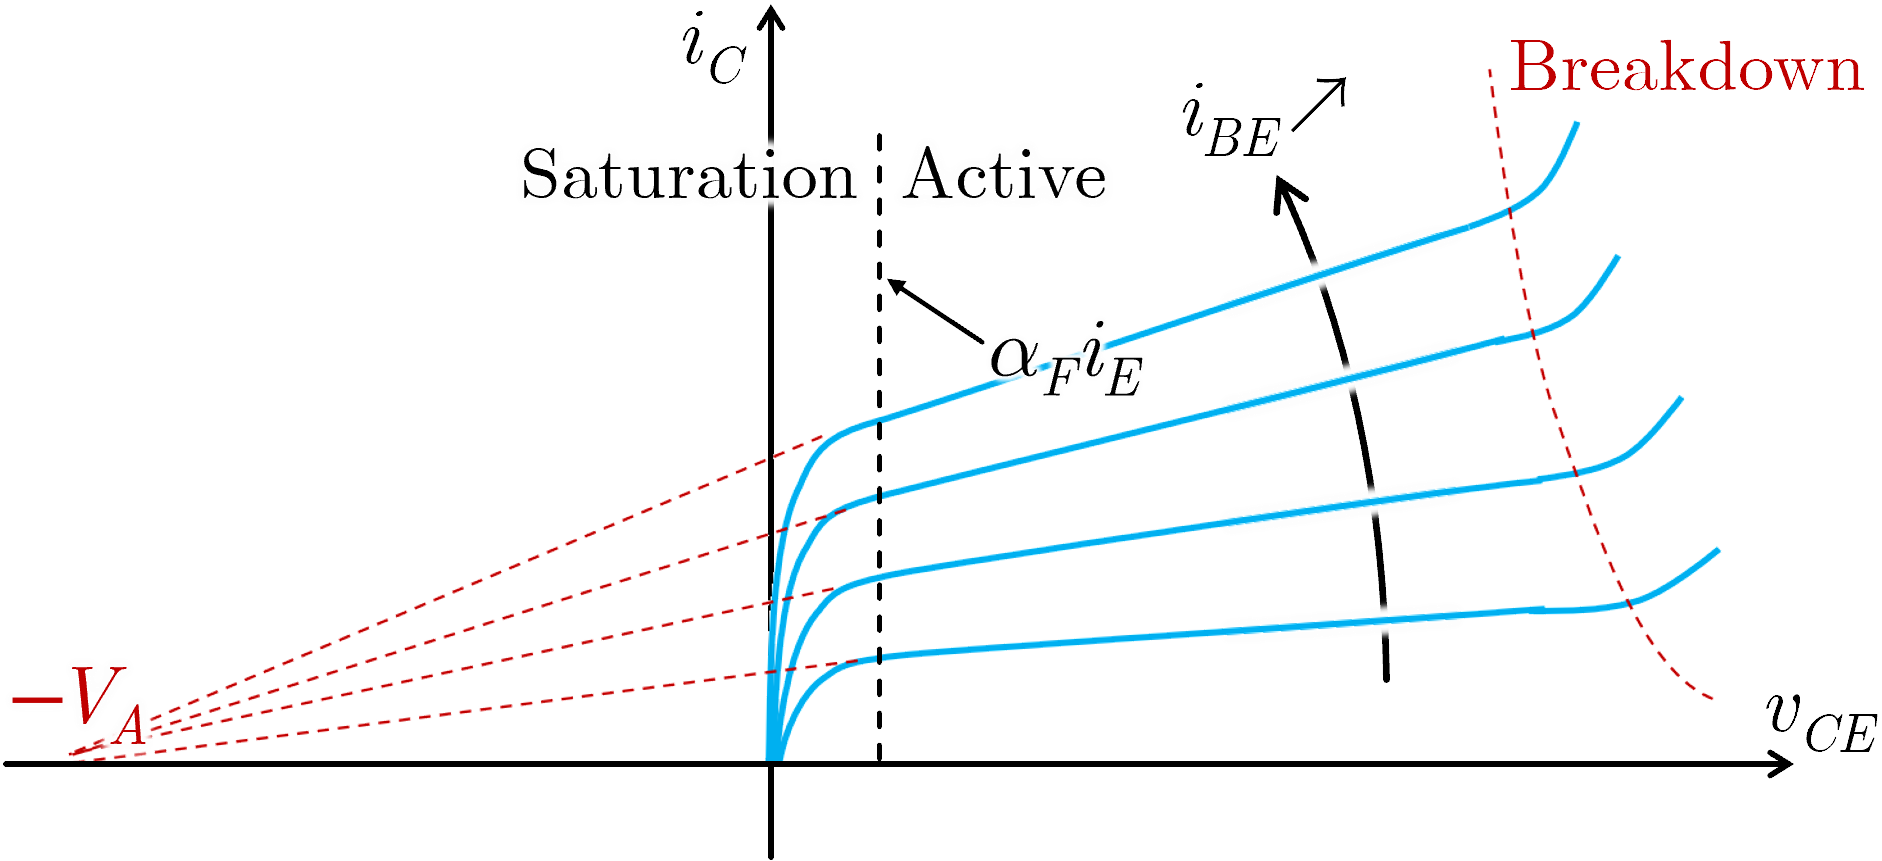
\includegraphics[width=7.25cm]{Early.png}
	\caption{考虑Early效应时\textsl{npn}型BJT的$i_C-v_{CE}$特性曲线}
	\vspace{-1em}
\end{figure}

Early效应产生自Active模式下\textbf{从集电极看去的电阻不为无穷},即集电极的流控流源上并联有电阻$r_0$。对$i_C=I_S\e^{v_{BE}/V_T}\left(1+\dfrac{v_{CE}}{V_A}\right)$求导,有 
$$r_0 = \left(\left.\dfrac{\partial i_C}{\partial v_{CE}}\right|_{v_{BE}}\right)^{-1} = \dfrac{V_A+V_{CE}}{I_C} \approx \dfrac{V_A}{I_C}$$

\begin{figure}[ht!]
	\begin{center}
	\cbox{
		\draw (0,0) node[left](B){B} to[short, o-, f=$i_B$] ++(1.1,0) to[short, -*] ++(0.4,0) coordinate(BJT);
		\draw (1.5,1.5) node[left](C){C} to[short, o-, f>^=$i_C$] ++(0,-0.6) coordinate(r0) to[cI, l=$\alpha_F i_E$] (BJT)
		(r0) to[short, *-] ++(1.5,0) coordinate(r1) to[R, l=$r_0$] (BJT -| r1) -- (BJT);
		\draw (BJT) to[Do, l=$D_E$] ++(0,-0.9) to[short, -o, f^>=$i_E$] ++(0,-0.6) node[left]{E};
	}
	\vspace{-1em}
	\end{center}
	\caption{考虑Early效应的\textsl{npn}型BJT的Active模式模型}
\end{figure}

\textsl{npn}型BJT的$i_C-v_{CE}$上,Saturation 区域中更靠近$v_{CE}=0$的区域中曲线斜率会有明显的增大,这块区域称为 Deeper Saturation 区(深度饱和区)。此区域中,不同于先前的\textbf{大信号\,$\symbf{\beta}$}($\beta_\mrm{DC}=\dfrac{I_C}{I_B}=\beta_F$),定义\textbf{小信号\,$\symbf{\beta}$}为$\beta_\mrm{AC}=\dfrac{\Dif i_C}{\Dif i_B}\bigg|_{v_{CE}}$、\textbf{强制\,$\symbf{\beta}$}为$\beta_{\symup{forced}}=\dfrac{i_C}{i_B}\bigg|_{v_{CE}}$,这两个$\beta$比大信号\,$\beta$小不少。

此外,深度饱和区中,可以近似有$v_{CE\symup{sat}}=v_{CE\symup{off}}+I_{C\symup{sat}}R_{CE\symup{sat}}$,其中$R_{CE\symup{sat}}=\dfrac{\partial v_{CE}}{\partial i_C}\bigg|_{i_B=I_B \atop i_C=I_{C\symup{sat}}}$。

\textbf{一般取临界饱和区$\symbf{V_{CE\symbfup{sat}}}\symbfup{=0.3\,V}$,深度饱和区$\symbf{V_{CE\symbfup{sat}}}\symbfup{=0.2\,V}$。}

\paragraph{BJT的传递特性}

\textsl{npn}型BJT的传递特性,一般考虑的是$v_{CE}-v_{BE}$传递特性。
在 Cutoff 模式,$v_{BE}< v_{BE\symup{on}}$;
在 Saturation 模式,$v_{BE} > v_{BE\symup{on}}$,$v_{BC} = v_{BE} - v_{CE} > v_{BC\symup{on}}$,$v_{CE}$电压也呈水平,电压值下降至$v_{CE\mrm{sat}}$;
在 Active 模式下,$v_{BE} > v_{BE\symup{on}}$,$v_{BC} = v_{BE} - v_{CE} < v_{BC\symup{on}}$。
一般取这两个阈值电压$v_{BE\symup{on}}=0.5\symup{\,V},v_{BC\symup{on}}=0.4\symup{\,V}$。

\begin{wrapfigure}{r}{2cm}
	\vspace{-2.5em}\raggedleft
	\cbox{
		\draw (0,0) to[open, o-, v=$v_{\mrm{in}}$] (0,-1) coordinate(GND) node[ground]{}
		(0,0) to[short, o-] ++(0.5,0) node[npn, anchor=B](BJT){}
		(BJT.E) -- (GND -| BJT.E) node[ground]{}
		(BJT.C) to[short, f<=$i_C$] ++(0,0.5)
		to[R, l_=$R_C$] ++(0,1) node[vcc]{$V_{dd}$}
		(BJT.C) ++(0,0.2) to[short, *-o] ++(0.5,0) coordinate(C)
		to[open, o-, v=$v_{\mrm{out}}$] (GND -| C) node[ground]{}
		;
	}
	\vspace{-2.5em}
\end{wrapfigure}
考虑在如右电路中进行定量分析:
\begin{itemize}
	\item $v_{BE}< v_{BE\symup{on}}$时,BJT工作在 Cutoff 模式,$i_C=0$,$v_{\mrm{out}}=v_{CE}=V_{dd}$;
	\item $v_{BE} > v_{BE\symup{on}}$,$v_{BC} = v_{BE} - v_{CE} < v_{BC\symup{on}}$时,BJT工作在 Active 模式下,有$i_C=I_S\e^{v_{BE}/V_T}$,则$v_{\mrm{out}}=V_{dd}-i_CR_C=V_{dd}-R_CI_S\e^{v_{\mrm{in}}/V_T}$;
	\item $v_{BC} = v_{BE} - v_{CE} = v_{\mrm{in}} - v_{\mrm{out}} > v_{BC\symup{on}}$时,即$v_{\mrm{out}} < v_{\mrm{in}} - v_{BC\symup{on}}$时,BJT工作在 Saturation 模式,$v_{\mrm{out}}=V_{CE\mrm{sat}}$,$I_{C\mrm{sat}}=\dfrac{V_{dd}-V_{CE\mrm{sat}}}{R_C}$。
\end{itemize}

\subsubsection{BJT直流分析}

BJT工作在 Cutoff 模式下和 Saturation 模式下时,其通断行为为一个受$v_{\mrm{in}}$控制的开关。

BJT工作在 Active 模式时,若直接解KVL、KCL方程,由于有$I_C=I_S\e^{\textstyle\frac{v_{BE}}{V_T}}$等超越式,方程一般没有解析解。\textbf{一般取$\symbf{|V_{BE}|}\symbfup{=0.7\,V}$},替代超越式列方程求解。

\subsubsection{BJT交流分析}

在$v_{BE}-v_{CE}$传递曲线中,Active模式区域中有一段斜率变化不大的曲线。加直流偏置电压$V_{BE}$偏置到该区域中\tboba{静态工作点}~$Q$,然后加交流小信号,则输出的交流成分是交流小信号依$Q$处斜率的放大信号,增益可有估计
$$A_v=\dfrac{\dif v_o}{\dif v_{in}}\bigg|_{v_{in}=V_{BE}}=-\dfrac{1}{V_T}R_CI_S\e^{v_{BE}/V_T}=-\dfrac{I_CR_C}{V_T}=-\dfrac{V_{dd}-V_{CE}}{V_T}>-\dfrac{V_{dd}-V_{CE\text{sat}}}{V_T}$$

偏置点$Q$的选取,或者说偏置电压$V_{BE}$的取值,对上面所述的放大过程十分重要。

\textbf{定量分析}\quad 设BE上输入电压$v_{in}=V_{BE}+v_{be}\sin(\omega t+\varphi)$,则由Active模式电流关系即有
\begin{align*}
	i_C&=I_S\e^{V_T^{-1}v_{BE}}
	=I_S\e^{V_T^{-1}\left(V_{BE}+v_{be}\sin(\omega t+\varphi)\right)}
	\xlongequal{I_C=I_S\e^{V_T^{-1}V_{BE}}} I_C\e^{V_T^{-1}v_{be}\sin(\omega t+\varphi)}\\[-3pt]
	&\xlongequal{v_{be} \ll V_T} I_C\left(1+\dfrac{1}{V_T}v_{be}\sin(\omega t+\varphi)\right)
	=I_C+\dfrac{I_C}{V_T}v_{be}\sin(\omega t+\varphi)
\end{align*}
定义电路的\tboba{跨导}值
\equ{
	g_m=\dfrac{I_C}{V_T}=\dfrac{\partial i_C}{\partial v_{BE}}\bigg|_{i_C=I_C}
}
\noindent 进一步,代入可求
$$v_o=V_{dd}-i_CR_C=V_{dd}-I_CR_C-\dfrac{I_C}{V_T}R_Cv_{be}\sin(\omega t+\varphi)=V_{CE}-g_mR_Cv_{be}\sin(\omega t+\varphi)$$
于是
\equ{
	A_v=\dfrac{v_o\big|_\text{AC}}{v_{in}\big|_\text{AC}}=-g_mR_C
}

考虑自输入端(基极)看去的输入阻值,其为$R_\mrm{in}=\dfrac{\symup{\Delta} v_\mrm{in}}{\symup{\Delta} i_\mrm{in}}=\dfrac{\symup{\Delta} v_{BE}}{\symup{\Delta} i_B}$。
由$i_B=\dfrac{i_{C}}{\beta}=\dfrac{I_{C}}{\beta}+\dfrac{1}{\beta}\dfrac{I_{C}}{V_{T}}v_\mrm{in,AC}$,知$\symup{\Delta} i_{B}=\dfrac{1}{\beta}\dfrac{I_{C}}{V_{T}}v_\mrm{in,AC}=\dfrac{1}{\beta}g_{m}v_\mrm{AC}$,进而有
\equ{
	R_{in}=\dfrac{\symup{\Delta} v_{BE}}{\symup{\Delta} i_{B}}=\dfrac{v_\mrm{in,AC}}{\symup{\Delta} i_{B}}=\dfrac{V_{T}}{I_{B}}=\dfrac{\beta}{g_{m}}
}


\subsection{金属—氧化物—半导体场效应晶体管(MOSFET)}

\ctikzset{tripoles/mos style/arrows}
\ctikzset{tripoles/pmos style/nocircle}
\bu[MOSFET]{
	\cbox{\draw[color=balib] (0,0) node[nmos, bulk]{};}(\texttt{nmos, bulk})
	\cbox{\draw[color=balib] (0,0) node[pmos, bulk]{};}(\texttt{pmos, bulk})
}{}

\subsubsection{MOSFET的结构与原理}

\subsubsection{MOSFET的端口特性}

\paragraph{$\symbf{i_D-v_{DS}}$特性}

随$v_{DS}$增大,在沟道夹断之前$i_D$不断增大,直到$v_{GS}-v_{DS}=V_{th}$后沟道夹断,$i_D$不再变化。达到$v_{GS}-v_{DS}=V_{th}$之前,称该NMOS管工作在\textbf{Triode区}(「三极管区」);达到$v_{GS}-v_{DS}=V_{th}$之后,称该NMOS管工作在\textbf{Saturation区}(「饱和区」)。

在 Triode区,有 
\equ{
	i_D=\mu_\textsl{n}C_\text{ox} \dfrac{W}{L } \left[(v_{GS}-V_{th})v_{DS}-\dfrac{1}{2}v_{DS}^2\right] \label{Eq: MOS-T}
}
其中$\dfrac{W }{L }$即沟道的宽高比;基于这个式子,定义\textbf{过驱动电压}$v_\mrm{OV}=v_{GS}-V_{th}$,\tboba{跨导参数}~$k_\textsl{n} = \mu_\textsl{n}C_\text{ox} \dfrac{W}{L }$。当$v_{DS} \to 0$时,略去高次小项,上式变为$i_D=\mu_\textsl{n}C_\text{ox} \dfrac{W}{L } (v_{GS}-V_{th})v_{DS} = k_\textsl{n}(v_{GS}-V_{th})v_{DS}$,于是可以定义此时NMOS管的等效电阻$r_{DS}=\dfrac{1}{k_\textsl{n}(v_{GS}-V_{th})}$。

在 Saturation区,$i_D$将保持两区交界处的饱和值,即向\ref{Eq: MOS-T}式代入$v_{DS} = v_{DS\mrm{sat}} = v_{GS}-V_{th}$,有 
\equ{
	i_D=\dfrac{1}{2}\mu_\textsl{n}C_\text{ox} \dfrac{W}{L } (v_{GS}-V_{th})^2
}
实际上,Saturation区沟道夹断之后还会随$v_{DS}$增大继续缩短,即会有
\begin{align*}
	i_D &= \dfrac{1}{2}\mu_\textsl{n}C_\text{ox} \dfrac{W}{L-\Dif L} (v_{GS}-V_{th})^2
	= \dfrac{1}{2}\mu_\textsl{n}C_\text{ox} \dfrac{W}{L\left( 1-\dfrac{\Dif L}{L} \right)} (v_{GS}-V_{th})^2 \\
	&\xlongequal{\Dif L \ll L} \dfrac{1}{2}\mu_\textsl{n}C_\text{ox} \dfrac{W}{L}\left( 1+\dfrac{\Dif L}{L} \right) (v_{GS}-V_{th})^2
\end{align*}
而$\Dif L \propto v_{DS}$,设比例系数为$\dfrac{1}{V_A}$,则
\equ{
	i_D=\dfrac{1}{2}\mu_\textsl{n}C_\text{ox} \dfrac{W}{L } (v_{GS}-V_{th})^2\left( 1+\dfrac{v_{DS}}{V_A} \right)
}
这称为\tbome{沟道长度调制效应},也沿用BJT中的名词称为\textbf{Early效应},其中$V_A$称为\textbf{Early电压}。考虑Early效应时,Saturation区各$v_{GS}$下的$i_D-v_{DS}$曲线(直线)相交于$v_{DS}=-V_A$处。

\paragraph{$\symbf{i_D-v_{GS}}$特性}

固定$v_{DS}$,则由上知$i_D-v_{GS}$关系为
$$i_D = \begin{cases}[ll]
	0,& v_{GS}<V_{th},\\
	\dfrac{1}{2}k_n (v_{GS}-V_{th})^2,& V_{th} < v_{GS} < V_{th} + v_{DS},\\
	k_n \left[(v_{GS}-V_{th})v_{DS}-\dfrac{1}{2}v_{DS}^2\right],& v_{GS} > V_{th} + v_{DS}\text{。}
\end{cases}$$
其中,通常更重要的是$v_{GS}<V_{th}+v_{DS}$,即在 Saturation区中的部分。

\paragraph{$\symbf{v_{DS}-v_{GS}}$特性}

基于图~\ref{Pic: NMOS tran circuit}~所示电路,由前面的伏安特性容易得到$v_{DS}-v_{GS}$关系,其可分为 Cutoff、Saturation、Triode三个区,如图~\ref{Pic: NMOS tran}~所示。

\begin{figure}[ht!]
	\centering
	\subfloat[电路]{\label{Pic: NMOS tran circuit}
		\begin{circuitikz}
			\draw (0,0) coordinate(I) 
			to[short, o-] ++(0.5,0) node[nmos, anchor=G](T){}
			(T.S) 
			-- ++(0,-0.5) node[ground](GND){}
			(T.D) 
			to[short, i<=$i_D$, !vi, name=iD] ++(0,0.5) coordinate(O) 
			to[R, l=$R_D$] ++(0,1) node[vcc]{$V_{dd}$}
			(I) 
			to[open, o-o, v=$v_{GS}$] (GND -| I) node[ground]{}
			(O) 
			to[short, -o] ++(0.5,0) coordinate(O1) 
			to[open, o-o, v=$v_{DS}$] (GND -| O1) node[ground]{}
			;
			\bi{iD}
		\end{circuitikz}
	}
	\qquad
	\subfloat[特性曲线]{\label{Pic: NMOS tran}
		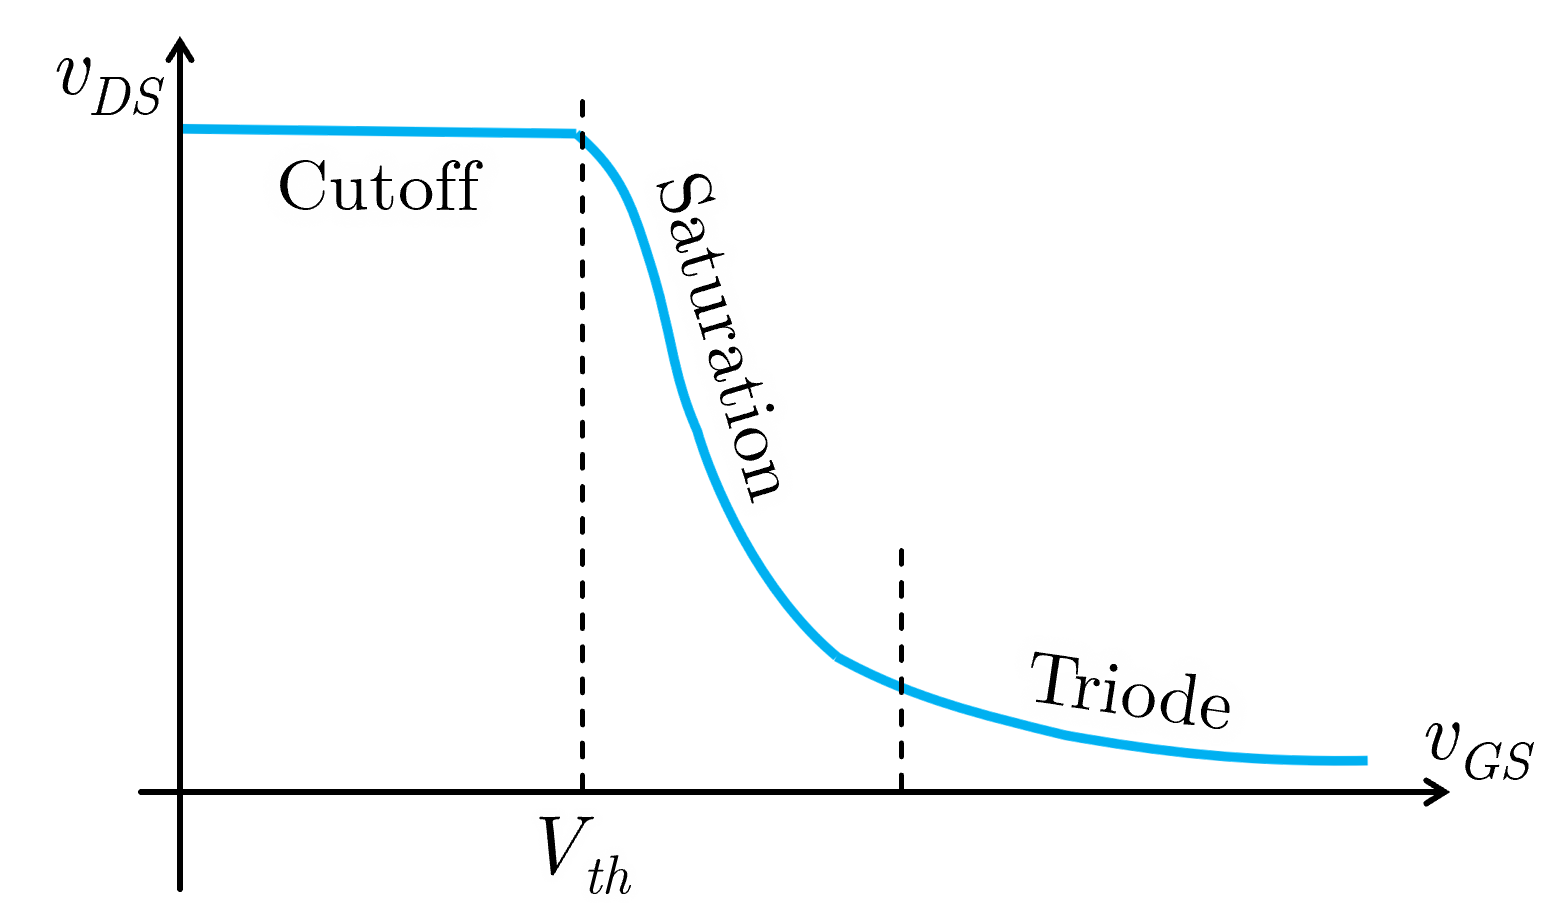
\includegraphics[width=6.03cm]{MOS_vDS-vGS.png}
	}
	\caption{NMOS管的$v_{DS}-v_{GS}$特性}
\end{figure}

\subsubsection{MOSFET的交流增益}

在$v_{DS}-v_{GS}$传递曲线中,Saturation区域中有一段斜率变化不大的曲线。加直流偏置电压$V_{GS}$偏置到该区域中\tboba{静态工作点}~$Q$,然后加交流小信号,则输出的交流成分是交流小信号依$Q$处斜率的放大信号。

在 Saturation区内,据晶体管的特性有
\begin{align*}
	i_D &= \dfrac{1}{2} k_\textsl{n} (V_{GS} + v_{\mrm{in,AC}} - V_{th})^2 
	= \dfrac{1}{2} k_\textsl{n} (V_{GS} - V_{th})^2 + k_\textsl{n} (V_{GS} - V_{th})v_{\mrm{in,AC}} + \dfrac{1}{2} k_\textsl{n} v_{\mrm{in,AC}}^2 \\
	&\xlongequal{\frac{1}{2} v_{\mrm{in,AC}} \ll V_{GS} - V_{th}}
	I_D + k_\textsl{n} (V_{GS} - V_{th})v_{\mrm{in,AC}}
\end{align*}
其中定义\tboba{跨导}参数为
\equ{
	g_m=k_\textsl{n}(v_\mrm{in}-V_{th})
}
基于图~\ref{Pic: NMOS tran circuit}~所示电路,由$v_\mrm{out}=V_{dd}-\dfrac{1}{2}k_\textsl{n}(v_\mrm{in}-V_{th})^2 R_D$,即有电压增益
$$A_v = \dfrac{\dif v_\mrm{out}}{\dif v_\mrm{in}}\bigg|_{v_\mrm{in}=V_{GS}}
= -k_\textsl{n}(v_\mrm{in}-V_{th})R_D = -g_mR_D$$

NMOS管的小信号混合$\pi$模型如图~\ref{Pic: NMOS hybrid-pi}。
\begin{figure}[ht!]
	\centering
	\subfloat[简化混合$\pi$模型]{
		\begin{circuitikz}
			\fill [fill=white!95!black, rounded corners] (1.2,0.3) rectangle (3.3,-1.8); 
			\draw (0,0) node[left](G){$G$} 
			to[short, o-o] ++(1.5,0)
			to[open, o-o, v=$v_{gs}$] ++(0,-1.5)
			to[short, o-] ++(0.75,0) coordinate(S)
			to[short, -o] ++(0,-0.5) node[below]{$S$}
			(S) -- ++(0.75,0) 
			to[cI, l=$g_mv_{gs}$, invert] ++(0,1.5)
			to[short, -o] ++(1.5,0) node[right]{$D$}
			;
		\end{circuitikz}
	}
	\qquad
	\subfloat[考虑沟道长度调制效应的混合$\pi$模型]{
		\begin{circuitikz}
			\fill [fill=white!95!black, rounded corners] (1.2,0.3) rectangle (4.3,-1.8); 
			\draw (0,0) node[left](G){$G$} 
			to[short, o-o] ++(1.5,0)
			to[open, o-o, v=$v_{gs}$] ++(0,-1.5)
			to[short, o-] ++(0.75,0) coordinate(S)
			to[short, -o] ++(0,-0.5) node[below]{$S$}
			(S) -- ++(0.75,0) 
			to[cI, l=$g_mv_{gs}$, invert] ++(0,1.5) -- ++(1,0)
			(S) -- ++(1.75,0) to[R, l_=$r_o$] ++(0,1.5)
			to[short, -o] ++(1.5,0) node[right]{$D$}
			;
		\end{circuitikz}
	}
	\caption{小信号混合$\pi$模型}\label{Pic: NMOS hybrid-pi}
\end{figure}

\subsubsection{MOSFET的频率响应}

如图~\ref{Pic: MOS CS Amp}~所示是一个典型的CS放大电路,其中$C_1$,$C_2$称为\textbf{耦合电容},$C_S$称为\textbf{旁路电容},它们起到为交流输入信号「隔直」的作用。但对低频交流信号,隔直电容并不能完全看作导线,从而对低频增益造成影响。

\begin{figure}[ht!]
	\centering 
	\cbox{
		\draw (0,0) node[nmos, anchor=G](MOS){}
			-- ++(-0.5,0) coordinate(G) 
			to[R, l=$R_G$] ++(0,-2) node[ground](GND){}
		(G)	-- ++(-0.5,0) 
			to[C, l=$C_1$] ++(-1,0)
			to[R, l=$R_\mrm{sig}$] ++(-1,0)
			to[V, l_=$v_\mrm{sig}$] ++(0,-2) node[ground]{}
		(MOS.S) to[I] (GND -| MOS.S) 
			-- ++(0,-0.2) node[vee]{$-V_{ss}$}
		(MOS.S) -- ++(1.5,0) coordinate(S)
			to[C, l=$C_S$] (GND -| S) node[ground]{}
		(MOS.D) to[short, f<=$i_D$, !vi, name=iD] ++(0,0.5)
			to[R, l=$R_D$] ++(0,1) node[vcc]{$V_{dd}$}
		(MOS.D) to[C, l=$C_2$] ++(1,0)
			-- ++(1.5,0) coordinate(O)
			to[R, l=$R_L$] ++(0,-2) node[ground]{}
		(O) to[short, -o] ++(0.5,0) node[right]{$v_o$}
		;
		\bf{iD}
	}
	\caption{一个典型的CS放大电路}\label{Pic: MOS CS Amp}
\end{figure}

\begin{itemize}
	\item 考虑$C_1$的作用,有 
	$$	v_{G}=\frac{R_G}{R_{sig}+\dfrac1{sC_1}+R_G}v_{sig} 
		=v_{sig}\frac{R_G}{R_{sig}+R_G}\mbome{\frac s{s+\dfrac1{C_1(R_{sig}+R_G)}}}
	$$
	其向电路传函贡献了一个高通项,零点$\omega_{L1} = \dfrac{1}{C_1(R_{sig}+R_{G})}$。
	\item 考虑$C_2$的作用,有
	$$	v_{out}=-i_{d}\frac{R_{D}R_{L}}{R_{D}+R_{L}+\dfrac{1}{sC_{2}}}
		=-i_{d}R_{L}\mbome{\frac{s}{s+\dfrac{1}{C_{2}(R_{D}+R_{L})}}}
	$$
	其也向电路传函贡献了一个高通项,零点$\omega_{L2} = \dfrac{1}{C_2(R_{D}+R_{L})}$。
	\item 考虑$C_S$的作用,有 
	$$	v_G - g_m v_{gs} \dfrac{1}{sC_S} = v_{gs} \quad\Longrightarrow\quad
		v_{gs} = v_G \mbome{\dfrac{s}{s + \dfrac{g_m}{C_S}}}
	$$
	其也向电路传函贡献了一个高通项,零点$\omega_{L3} = \dfrac{g_m}{C_S}$。
\end{itemize}

在高频部分,MOS管栅极和衬底极之间的氧化物电容将导通,不再有$i_G=0$,此时NMOS管的高频小信号模型如图~\ref{Pic: NMOS hybrid-pi at high-f}~所示,其中相比于一般小信号模型所多出的两个电容$C_{gs}$、$C_{gd}$将对高频增益造成影响。将图~\ref{Pic: MOS CS Amp}~改写为高频交流形式如图~\ref{Pic: MOS CS Amp AC},注意到
\begin{figure}[ht!]
	\centering
	\begin{circuitikz}[voltage shift=-0.4]
		\fill [fill=white!95!black, rounded corners] (0.6,0.6) rectangle (4.8,-1.8); 
		\draw (0,0) node[left](G){$G$} 
			to[short, o-] ++(1.5,0) coordinate(g)
			to[C, l=$C_{gs}$, v=$v_{gs}$] ++(0,-1.5)
			-- ++(1,0) coordinate(S)
			to[short, -o] ++(0,-0.5) node[below]{$S$}
		(S) -- ++(1,0) 
			to[cI, l=$g_mv_{gs}$, invert] ++(0,1.5) coordinate(d)
			-- ++(1,0)
		(g) to[C, l=$C_{gd}$] (d)
		(S) -- ++(1.75,0) to[R, l_=$r_o$] ++(0,1.5)
			to[short, -o] ++(1.2,0) node[right]{$D$}
		;
	\end{circuitikz}
	\caption{高频小信号混合$\pi$模型}\label{Pic: NMOS hybrid-pi at high-f}
\end{figure}
\begin{figure}[ht!]
	\centering 
	\cbox{
		\fill [fill=white!95!black, rounded corners] (0.6,0.6) rectangle (4.8,-1.8); 
		\draw (0,0) coordinate(MOSG) node[above]{$G$} 
			to[short, o-] ++(1.5,0) coordinate(g)
			to[C, l=$C_{gs}$, v=$v_{gs}$] ++(0,-1.5)
			-- ++(1,0) coordinate(mosS)
			to[short, -o] ++(0,-0.5) coordinate(MOSS) node[left]{$S$}
		(mosS) -- ++(1,0) 
			to[cI, l=$g_mv_{gs}$, invert] ++(0,1.5) coordinate(d)
			-- ++(1,0)
		(g) to[C, l=$C_{gd}$] (d)
		(mosS) -- ++(1.75,0) to[R, l_=$r_o$] ++(0,1.5)
			to[short, -o] ++(1.2,0) coordinate(MOSD) node[below]{$D$}
		(MOSG) -- ++(-1,0) coordinate(G) 
			to[R, l=$R_G$] ++(0,-1.5) node[ground](GND){}
		(G)	to[C, l=$C_1$] ++(-1,0)
			to[R, l=$R_\mrm{sig}$] ++(-1,0) -- ++(-0.3,0)
			to[V, l_=$v_\mrm{sig}$] ++(0,-1.5) node[ground]{}
		(MOSS) to[I] ++(0,-1.2) node[vee]{$-V_{ss}$}
		(MOSS) -- ++(1.5,0) coordinate(S)
			to[C, l=$C_S$] ++(0,-1) node[ground]{}
		(MOSD) -- ++(0,0.2) 
			to[short, f<=$i_D$, !vi, name=iD] ++(0,0.3)
			to[R, l=$R_D$] ++(0,1) node[vcc]{$V_{dd}$}
		(MOSD) to[C, l=$C_2$] ++(1.5,0) coordinate(O)
			to[R, l=$R_L$] ++(0,-1.5) node[ground]{}
		(O) to[short, -o] ++(0.5,0) node[right]{$v_o$}
		;
		\bf{iD}
		\draw[meihong!75!black, -latex, thick] (-0.5,-2.5) node[right]{$\mbome{C_{\symbfup{in}}}$} -- ++(0,3.5) -- ++(0.5,0);
	}
	\caption{图~\ref{Pic: MOS CS Amp}~中CS放大电路的高频交流等效形式}\label{Pic: MOS CS Amp AC}
	\vspace{-1.5em}
\end{figure}
\begin{align*}
	& v_\mrm{out} = (-g_m v_{gs} + i_{gd}) \cdot (R_L \parallel R_D \parallel r_o )
	\xlongequal[R_L' := R_L \parallel R_D \parallel r_o]{g_m v_{gs} \gg i_{gd}} -g_m v_{gs} R_L' \\[-5pt]
	&\Longrightarrow\quad i_{gd}=(v_{gs}-v_\mrm{out})sC_{gd}=(1+g_{m}R_{L}')sC_{gd}v_{gs}\\[-5pt]
	&\Longrightarrow\quad i_\mrm{in}=i_{gs}+i_{gd}=\left(C_{gs}+C_{gd}(1+g_{m}R_{L}')\right)sv_{gs}
\end{align*}
即可定义$C_\mrm{in} = C_{gs}+C_{gd}(1+g_{m}R_{L}')$,进而 
\begin{equation*}
	G_{v} =\dfrac{v_{o}}{v_\mrm{sig}}=\dfrac{-g_{m}v_{gs}R_{L}'}{v_\mrm{sig}}
	=\dfrac{-g_{m}R_{L}'}{v_\mrm{sig}}\dfrac{v_{G\_TH}}{1+sR_{G\_TH}C_\mrm{in}}
	=-\frac{g_{m}R_{L}'R_{G}}{R_\mrm{sig}+R_{G}}\mbome{\dfrac{1}{1+sR_{G\_TH}C_\mrm{in}}}
\end{equation*}
其中$R_{G\_TH}=R_\mrm{sig} \parallel R_B$,$v_{G\_TH} = \dfrac{R_B}{R_\mrm{sig}+R_B} v_\mrm{sig}$,标红项$\dfrac{1}{1+sR_{G\_TH}C_\mrm{in}}$即是向电路增益贡献的低通项,极点$\omega_{H1} = \dfrac{1}{R_{G\_TH}C_\mrm{in}}$。

\subsection{晶体管模块实例}

\subsubsection{电流镜}

最简单的电流镜形式如图~\ref{Pic: Simple C-mirror}~所示。其中,不考虑Early效应,若做到两个BJT完全相同,即$\beta_{Q_1} = \beta_{Q_2} =\beta$,就有
$$I_\mrm{ref} = I_{C1} + I_{B1} + I_{B2} = I_{C1} + \dfrac{I_{C1}}{\beta} + \dfrac{I_{C2}}{\beta} \xlongequal{I_\mrm{out} = I_S\e^\frac{v_{BE}}{V_T}} \left( 1+ \dfrac{2}{\beta} \right) I_\mrm{out} \quad \Longrightarrow \quad \dfrac{I_\mrm{out}}{I_\mrm{ref}} = \dfrac{1}{1+ \dfrac{2}{\beta}}\xlongrightarrow{\beta \to \infty} 1$$
若$Q_2$的发射结面积是$Q_1$的$m$倍,即$I_{S2}=mI_{S1}$,则有
$$I_\mrm{ref} = I_{C1} + I_{B1} + I_{B2} = I_{C1} + \dfrac{I_{C1}}{\beta} + \dfrac{I_{C2}}{\beta} \xlongequal{I_\mrm{out} = I_{S2}\e^\frac{v_{BE}}{V_T}} \left(1+ \dfrac{1}{m\beta}+ \dfrac{1}{\beta}\right) I_\mrm{out} \quad \Longrightarrow \quad \dfrac{I_\mrm{out}}{I_\mrm{ref}} = \dfrac{1}{1+ \dfrac{1}{m\beta}+ \dfrac{1}{\beta}}\xlongrightarrow{\beta \to \infty} m$$
此即一个根据$I_\mrm{ref}$和$m$确定的电流源。写出小信号模型可知,其输出等效电阻即为$r_{o2}$,不考虑Early效应时可视为$R_\mrm{out}=\infty$。事实上,即使考虑 Early效应,也可算出$\dfrac{I_\mrm{out}}{I_\mrm{ref}} = \dfrac{m}{1+\dfrac{1+m}{\beta}}\left( 1 + \dfrac{V_\mrm{out} - V_{BE}}{V_{A2}} \right)$,只需控制$V_\mrm{out}=V_{BE}$即可在电流大小上与无 Early效应时一致。

\begin{figure}[ht!]
	\centering
	\subfloat[  ]{\label{Pic: Simple C-mirror}
		\begin{circuitikz}
			\draw (0,0) -- ++(0.5,0) node[npn, anchor=B](Q2){$Q_2$}
			(0,0) -- ++(-0.5,0) node[npn, anchor=B, xscale=-1](Q1){\ctikzflipx{$Q_1$}}
			(0,0) to[short, -o] ++(0,-0.3) 
				to[open, o-o, v=$v_{BE}$] ++(0,-1) node[ground](GND){}
				to[short, o-] (GND -| Q2.E) -- (Q2.E) 
			(GND) to[short, o-] (GND -| Q1.E) 
				-- (Q1.E) 
			(Q1.C) -- ++(0,0.2) coordinate(cb)
				-- (cb -| GND) -- (0,0)
			(cb) to[short, -o, i<=$I_\mrm{ref}$, !vi, name=ref] ++(0,0.8)
			(Q2.C) -- ++(0,0.4)
				to[short, i<=$I_\mrm{out}$, -o, !vi, name=out] ++(0.6,0) node[right]{$V_\mrm{out}$}
			;
			\bi{ref}\bi{out}
		\end{circuitikz}
	}
	\qquad
	\subfloat[  ]{\label{Pic: Another C-mirror}
		\begin{circuitikz}
			\draw (0,0) -- ++(0.5,0) node[npn, anchor=B](Q2){$Q_2$}
			(0,0) -- ++(-0.5,0) node[npn, anchor=B, xscale=-1](Q1){\ctikzflipx{$Q_1$}}
			(0,0) to[short, -o] ++(0,-0.3) 
				to[open, o-o, v=$v_{BE}$] ++(0,-1) node[ground](GND){}
				to[short, o-] (GND -| Q2.E) -- (Q2.E) 
			(GND) to[short, o-] (GND -| Q1.E) 
				-- (Q1.E) 
			(0,0) -- ++(0,0.2) node[npn, anchor=E](Q3){$Q_3$}
			(Q3.B) -- (Q3.B -| Q1.C) 
			(Q1.C) -- (Q3.B -| Q1.C) 
				to[short, -o, i<=$I_\mrm{ref}$, !vi, name=ref] ++(0,0.8)
			(Q2.C) -- ++(0,0.4)
				to[short, i<=$I_\mrm{out}$, -o, !vi, name=out] ++(0.6,0) node[right]{$V_\mrm{out}$}
			(Q3.C) -- ++(0,0.4) node[vcc]{$V_{dd}$}
			;
			\bi{ref}\bi{out}
		\end{circuitikz}
	}
	\qquad
	\subfloat[  ]{\label{Pic: New C-mirror}
		\begin{circuitikz}
			\draw (0,0) -- ++(0.5,0) node[npn, anchor=B](Q2){$Q_2$}
			(0,0) -- ++(-0.5,0) node[npn, anchor=B, xscale=-1](Q1){\ctikzflipx{$Q_1$}}
			(0,0) to[short, -o] ++(0,-0.3) 
				to[open, o-o, v=$v_{BE}$] ++(0,-1) node[ground](GND){}
				to[short, o-] (GND -| Q2.E) -- (Q2.E) 
			(GND) to[short, o-] (GND -| Q1.E) 
				-- (Q1.E) 
			(Q2.C) -- ++(0,0.2) coordinate(cb)
				-- (cb -| GND) -- (0,0)
			(Q1.C) -- ++(0,1)
				to[short, -o, i<=$I_\mrm{ref}$, !vi, name=ref] ++(0,0.8)
			(cb) -- ++(0,0.2) node[npn, anchor=E](Q3){$Q_3$}
			(Q3.B) -- (Q3.B -| Q1.C)
			(Q3.C) -- ++(0,0.2)
				to[short, i<=$I_\mrm{out}$, -o, !vi, name=out] ++(0.6,0) node[right]{$V_\mrm{out}$}
			;
			\bi{ref}\bi{out}
		\end{circuitikz}
	}
	\caption{BJT电流镜}
\end{figure}


\subsubsection{差分对}




\newpage
x
%----------------------------------------------------------
\end{document}